\title{Bras mécanique et sudoku}
\author{Laurent Tainturier \& Alphonse TERRIER}
\date{2016-2017}
\documentclass[12pt,a4paper]{report}
\usepackage[utf8]{inputenc}
\usepackage[T1]{fontenc}
\usepackage[francais]{babel}
\usepackage{hyperref}
\usepackage{lmodern}
\usepackage{graphicx}
\usepackage{listings}
\usepackage{enumitem}
\usepackage{stmaryrd}
\usepackage{array}
\usepackage{minted}
\usepackage{color}
\usepackage{float}
\usepackage[backend=biber, autolang=other, sorting=none, style=science]{biblatex}
\usepackage[left=4cm,right=3cm,top=2.5cm,bottom=2.5cm]{geometry}
\usepackage{fancyvrb}
\frenchbsetup{StandardLists=true}
\newtheorem{theo}{Définition}[section]
\definecolor{lightgray}{gray}{.6}
\usepackage[dvipsnames]{xcolor}
\definecolor{yellow}{RGB}{225,220,0}

\newenvironment{changemargin}[2]{\begin{list}{}{%
\setlength{\topsep}{0pt}%
\setlength{\leftmargin}{0pt}%
\setlength{\rightmargin}{0pt}%
\setlength{\listparindent}{\parindent}%
\setlength{\itemindent}{\parindent}%
\setlength{\parsep}{0pt plus 1pt}%
\addtolength{\leftmargin}{#1}%
\addtolength{\rightmargin}{#2}%
}\item }{\end{list}}

\usepackage{placeins}



%\addbibresource{bibli.bib}

\begin{document}
\FloatBarrier

\begin{titlepage}
\begin{changemargin}{-1cm}{0cm}
	\centering
	\vspace{5cm}
	{\scshape\huge Institut Supérieur d'Électronique de Paris \par}
	\vspace{1cm}
	{\scshape\LARGE TIPE\par}
	\vspace{1.5cm}
	{\fontsize{45}{45}\selectfont\bfseries Le Rubik's Cube\par}
	\vspace{2cm}
	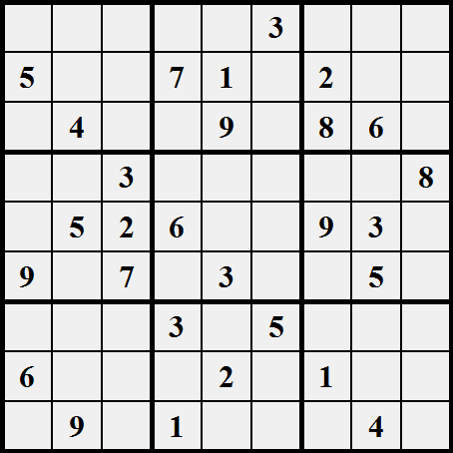
\includegraphics[width=0.7\textwidth]{../pictures/pagedegarde.png}\par\vspace{1.5cm}
	{\LARGE Laurent Tainturier \& Alphonse Terrier\par}
	\vfill
	\large supervisé par\par
	\large \bfseries M. Patrick COUVEZ

	\vfill


	{\large 2016-2017}
\end{changemargin}
\end{titlepage}

\tableofcontents
\addcontentsline{toc}{chapter}{Introduction}
\chapter*{Introduction}
	

	\chapter{Présentation du sudoku}
	
	\chapter{Électronique}
	\chapter{Mécanique}
	\chapter{Informatique}
	Tous les algorithmes sont implémentés en Python. Ils sont disponibles en annexe.
	\section{Résolution du sudoku}
	\section{Reconnaissance du sudoku}
	\section{Écriture et contrôle des moteurs}
	

\printbibliography
\nocite{*}
\appendix
\begin{changemargin}{-2cm}{-4cm}
\chapter{Fichier principal}
\label{main}
\inputminted[fontsize=\scriptsize, linenos=true]{Python}{../script/main.py}
\chapter{Script de résolution des sudokus}
\label{resolution}
\inputminted[fontsize=\scriptsize, linenos=true]{Python}{../script/resolution.py}
\chapter{Script de gestion de la caméra}
\label{camera}
\inputminted[fontsize=\scriptsize, linenos=true]{Python}{../script/camera.py}


\end{changemargin}
\end{document}
